        \section{Модель Хищник-Жертва Лотки-Вольтеры с учетом внутривидовой конкуренции}
         $\dot{u} = a u \left(1 - \frac{u}{k}\right)$ --- конкуренция за пищу.
         \begin{equation}
         \begin{cases}
         \dfrac{du}{dt} = au(t) - bu(t)v(t) - eu^2 \\[8pt]
         \dfrac{dv}{dt} = -cv(t) + du(t)v(t) - fv^2\\
         a,b,c,d,e,f > 0
         \end{cases}
\end{equation}
Введем те же безразмерные переменные: $\alpha, \beta, \gamma > 0$.
\begin{equation}
\begin{cases}
\dot{u} = u - uv - \alpha u^2\\
\dot{v} = -\gamma v + uv - \beta v^2
\end{cases}
\end{equation}             
       Неподвижные точки:
       \begin{gather*}
       u(1 - v - \alpha u) = 0\\
       v(-\gamma + u - \beta v) = 0\\
       O(0,0), \; N\left(\frac{1}{\alpha}, 0\right)\\
       M:\begin{cases}
       \alpha u + v = 1\\
       u - \beta v = \gamma
       \end{cases}\\
       \beta v = u - \gamma\\
       v = \frac{u}{\beta} - \frac{\gamma}{\beta}
\end{gather*}       
       
        \begin{enumerate}[label = \alph*)]
        \item $\gamma < \dfrac{1}{\alpha} \Rightarrow O, N, M$.
        \item $\gamma > \dfrac{1}{\alpha} \Rightarrow O, N$.
        \end{enumerate}
        $$J = \begin{pmatrix}
        1 - v - 2\alpha u & -u\\
        v & -\gamma + u - 2\beta v
\end{pmatrix}                
        $$
        $$J(O) = \begin{pmatrix}
        1 & 0\\
        0 & -\gamma
        \end{pmatrix}
        $$
        $\Rightarrow$ седло
        \begin{enumerate}[label = \alph*)]
        \item $$J(N) = \begin{pmatrix}
        -1 & -\frac{1}{\alpha}\\
        0 & -\gamma + \frac{1}{\alpha}
        \end{pmatrix}
        \Rightarrow
        $$
        $$\Rightarrow \begin{cases}
        \lambda_1 = -1\\
        \lambda_2 = -\gamma + \frac{1}{\alpha} > 0
        \end{cases}
        $$
        \end{enumerate}
        
        \begin{enumerate}[label = \alph*)]
        \item Седло
        \item Устойчивый узел (сток)
        \end{enumerate}
        \begin{gather*}
        J(M) = \begin{pmatrix}
        -\alpha u & -u\\
        v & -\beta v
        \end{pmatrix}\\
        \TrCh6 J(M) = -(\alpha u + \beta v) < 0\\
        |J(M)| = \alpha \beta v u + uv = (1 + \alpha \beta) uv > 0
        \end{gather*}
        $D = (\TrCh6 J(M))^2 - 4|J| < 0 \Rightarrow$  устойчивый фокус.    
        \section{Взаимодействие популяций двух конкурирующих видов}
          \begin{equation}
         \begin{cases}
         \dfrac{du}{dt} = au(t) - bu(t)v(t) - eu^2 \\[8pt]
         \dfrac{dv}{dt} = -cv(t) + du(t)v(t) - fv^2\\
         a,b,c,d,e,f > 0
         \end{cases}
\end{equation}
\begin{equation}
\begin{cases}
\dot{u} = r_1 u + a_{12} uv - a_{11} u^2\\
\dot{v} = r_2 v + a_{21} uv - a_{22} v^2
\end{cases}
\end{equation}
Классификация $(a_{12}, a_{21})$:
\begin{itemize}
\item Нейтрализм $(0, 0)$
\item Аменсализм $(-, 0)$
\item Коменсализм $(+, 0)$
\item Конкуренция $(-, -)$
\item Хищник - Жертва $(-, +)$
\item Мутуализм $(+, +)$
\end{itemize}
Введем те же безразмерные переменные:
\begin{gather*}
\begin{cases}
\dot{u} = u - uv - \alpha u ^2\\
\dot{v} = \gamma v - uv - \beta v^2
\end{cases}\\
u(1 - v - \alpha u) = 0\\
v(\gamma - u - \beta v) = 0\\
O(0,0), \;
N\left(\frac{1}{\alpha}, 0 \right), \;
P\left(0, \frac{\gamma}{\beta} \right),\\
M: \begin{cases}
\alpha u + v = 1\\
u + \beta v = \gamma
\end{cases}\\
\Delta = \alpha \beta - 1\\
\Delta u = \begin{vmatrix}
1 & 1\\
\gamma & \beta
\end{vmatrix} = \beta - \gamma\\
\Delta v = \begin{vmatrix}
\alpha & 1\\
1 & \gamma
\end{vmatrix} = \alpha \gamma - 1\\
u = \dfrac{\beta - \gamma}{\alpha \beta - 1}\\
v = \dfrac{\alpha \gamma - 1}{\alpha \beta - 1}
\end{gather*}
\begin{center}
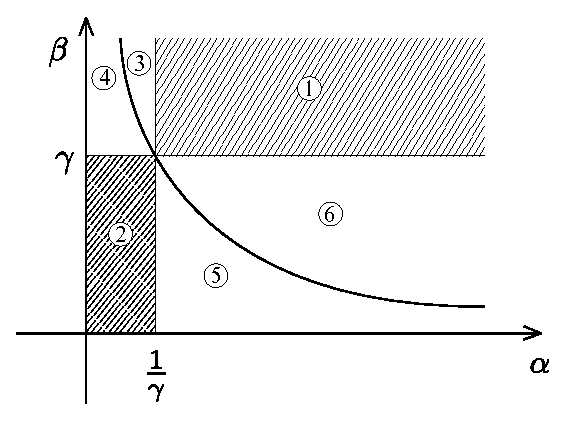
\includegraphics[width = 0.7\textwidth]{ch6/system.eps}
\end{center}
\begin{enumerate}
\item $\alpha \beta > 1, \; \beta > \gamma, \; \alpha \gamma > 1, (u > 0, v > 0)$
\item $\alpha \beta < 1, \; \beta < \gamma, \; \alpha \gamma < 1, (u > 0, v > 0)$
\end{enumerate}
$$J = \begin{pmatrix}
1 - v - 2 \alpha u & -u\\
-v & \gamma - u - 2\beta v
\end{pmatrix}
$$
\begin{enumerate}
\item $J(O) = \begin{pmatrix}
1 & 0\\
0 & \gamma
\end{pmatrix}$ --- неустойчивый узел.
\item $J(N) = \begin{pmatrix}
-1 & -\frac{1}{\alpha}\\
0 & \gamma - \frac{1}{\alpha}
\end{pmatrix}
$
\begin{enumerate}[label = \alph*)]
\item $\alpha \gamma > 1 \Rightarrow$ седло, области 1, 5, 6.\\
\item $\alpha \gamma < 1 \Rightarrow$ сток, области 2, 3, 4.\\
\end{enumerate}
\item $J(P) = \begin{pmatrix}
1 - \frac{\gamma}{\beta} & 0\\
\frac{\gamma}{\beta} & -\gamma
\end{pmatrix}$
\begin{enumerate}[label = \alph*)]
\item $\beta > \gamma \Rightarrow$ седло, области 1, 3, 4.
\item $\beta < \gamma \Rightarrow$ сток, области 2, 5, 6.
\end{enumerate}
\item $M\left(\frac{\beta - \gamma}{\alpha\beta - 1}, \frac{\alpha\gamma - 1}{\alpha \beta - 1}\right)$
\begin{gather*}
u^* = \frac{\beta - \gamma}{\alpha\beta - 1}\\
v^* = \frac{\alpha\gamma - 1}{\alpha \beta - 1}\\
J(M) = \begin{pmatrix}
-\alpha u^* & -u^*\\
-v^* & -\beta v^*
\end{pmatrix}\\
\TrCh6 J(M) = -\alpha u^* - \beta v^* < 0\\
|J(M)| = u^* v^* (\alpha \beta - 1)
\end{gather*}
\begin{enumerate}[label = \alph*)]
\item $\alpha \beta > 1 \Rightarrow$ устойчивое положение (например, устойчивый фокус), область 1.
\item$\alpha \beta < 1 \Rightarrow$ седло, область 2.
\end{enumerate}
\end{enumerate}
\begin{center}
\begin{tabular}{|c|c|c|c|c|c|c|}
\hline
Точки $\backslash$ Области & 1 & 2 & 3 & 4 & 5 & 6 \\ \hline
$N$ & седло & сток & сток & сток & седло & седло\\ \hline
$P$ & седло & сток & седло & седло & сток & сток\\ \hline
$M$ & устойчивое положение & седло & --- & --- & --- & --- \\ \hline
\end{tabular}\\[8pt]
\end{center}
Ниже представлен график для областей 3, 4.
\begin{center}
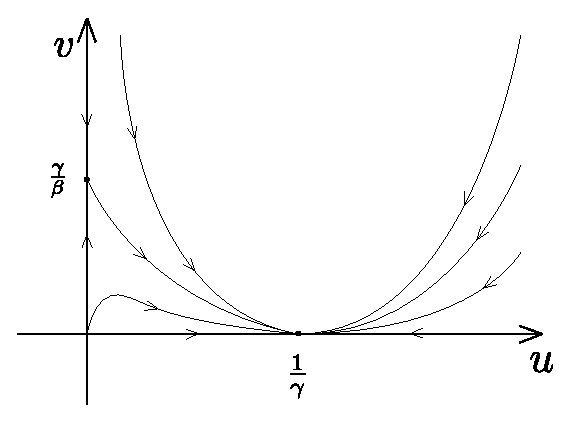
\includegraphics[width = 0.7\textwidth]{ch6/system(34).eps}\\[8pt]
Здесь вид $v$ вымирает, а вид $u$ --- выживает.\\[20pt]
\end{center}
Ниже представлен график для областей 5, 6.
\begin{center}
\includegraphics[width = 0.7\textwidth]{ch6/system(56).eps}\\
Здесь вид $u$ вымирает, а вид $v$ --- выживает.
\end{center}
Ниже представлен график для области 2.
\begin{center}
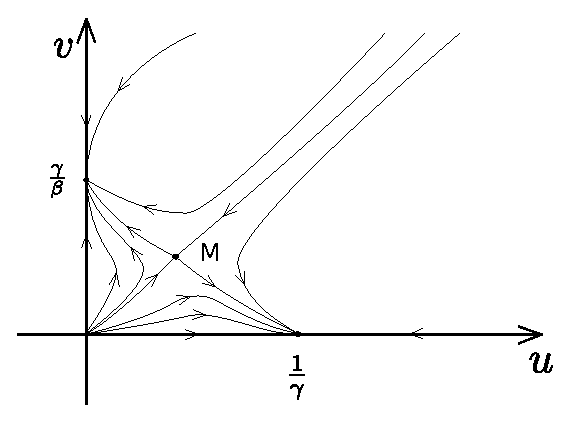
\includegraphics[width = 0.7\textwidth]{ch6/system(2).eps}\\
Здесь, если $(u_0, v_0)$ выше устойчивой сепаратриссы седла $M$, то $v$ побеждает, а $u$ --- погибает.
Если $(u_0, v_0)$ ниже устойчивой сепаратриссы седла $M$, то $u$ побеждает, а $v$ --- погибает.
\end{center}
Ниже представлен график для области 1.
\begin{center}
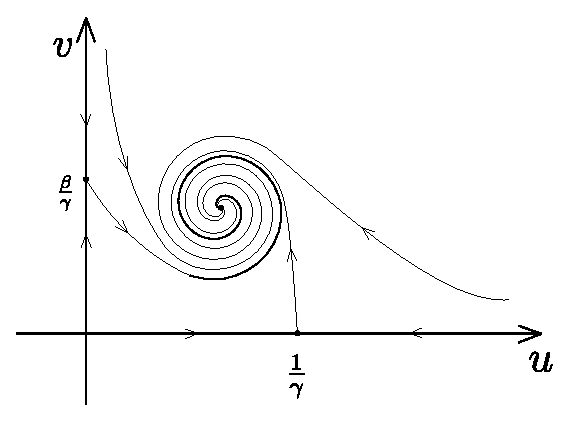
\includegraphics[width = 0.7\textwidth]{ch6/system(1).eps}\\
Здесь выживают оба вида.
\end{center}
Устойчивое состояние маловероятно для видов, занимающих общую нишу.
\section{Модель Гаузе}
\begin{equation}
\dfrac{\dot{u_i}}{u_i} = \sum_{k=1}^{m} b_{ik} R_k - \alpha_i, \; i = 1, 2, \dots, n
\end{equation}
$\alpha_i$ --- коэффциент смертности $i$-го вида.\\
$R_k$ --- изобилие $k$-го ресурса пищи.\\
$b_{ik}$ --- эффективность $i$-го вида в использовании $k$-го ресурса пищи.
$a_{kj}$ --- интенсивность поедания $k$-го ресурса $j$-ым видом.
\begin{equation}
R_k = \overline{R_k} - \sum_{j = 1}^{n} a_{kj} u_j
\end{equation}
$\overline{R_k}$ --- суммарный ресурс.\\[8pt]
Модель взаимодействия видов Гаузе:
\begin{equation}\label{gauzeCH6}
\dot{u_i} = u_i \sum_{k=1}^{m} b_{ik}(\overline{R_k} - \sum_{j = 1}^{n} a_{kj} u_j) - \alpha_i u_i, \; i = 1, 2, \dots, n.
\end{equation}
\begin{theorem}[Гаузе]
Пусть задана математическая модель (\ref{gauzeCH6}) (взаимодействие видов и пищи). Пусть $m<n$ (количество видов пищи меньше, чем количество видов). Тогда один вид вымирает.
\end{theorem}
\begin{proof}\\
Рассмотрим набор $c_1, \dots, c_n \in \SetR$ : 
$$\sum_{i=1}^{n} b_{ik} c_i = 0, \quad k = 1,\dots, m, \; m<n.$$
Получили систему линейных уравнений с матрицей $\SetR^{m\times n}, \; m<n$. Эта система имеет целое множество решений $\Sigma$. То есть $\exists (c_1, c_2, \dots, c_n) \in \Sigma$.\\
Тогда из $\Sigma$ всегда можно выбрать такой набор, что $\sum_{i=1}^{n} c_i \alpha_i \neq 0$.
$$-c = (-c_1, -c_2, \dots, -c_n) \in \Sigma, \text{если} c \in \Sigma.$$
Поэтому $c$ всегда можно выбрать так, чтобы $\sum_{i=1}^{k}c_i \alpha_i > 0.$\\
Рассмотрим $V = \sum_{i=1}^{n} c_i \log u_i(t)$, где $u_i(t)$ --- решения системы.
\begin{gather*}
\dot{V} = \sum_{i=1}^{n} c_i \frac{\dot{u_i}}{u_i} = \sum_{i=1}^{n} c_i \left( \sum_{k=1}^{m} b_{ik} R_k - \alpha_i \right) = \sum_{i = 1}^{n} c_i \sum_{k = 1}^{m} b_{ik} R_k - \sum_{i = 1}^{n} c_i \alpha_i =\\
= \sum_{k = 1}^{m} R_k \sum_{i = 1}^{n} b_{ik} c_i - \sum_{i = 1}^{n} c_i \alpha_i\\
\dot{V} = - \sum_{i = 1}^{n} c_i \alpha_i = -\alpha\\
\sum_{i=1}^{n} c_i \log u_i(t) = V = - \alpha t + \log|c|\\
\prod_{i = 1}^{n}(u_i)^{c_i} = c e^{-\alpha t}, \; \alpha>0\\
\end{gather*}
В последнем равенстве перейдем к пределу при $t \to +\infty$:
$$\prod_{i=1}^{n}(u_i)^{c_i} \to 0, \; t\to \infty. $$
Тогда найдется $i^* \in \{1, n\}$ такое, что 
$$\lim_{t \to \infty} u_i^*(t) = 0.$$
\end{proof}
\section{Модель загрязнение - окружающая среда}
\begin{equation}
\dot{P} = \alpha - bP
\end{equation}
\begin{equation}
\dot{E} = rE\left(1 - \dfrac{E}{k} \right)
\end{equation}
$P$ --- загрязнение.\\
$\alpha = \const$ --- интенсивность выбросов.\\
$E$ --- среда.
\begin{equation}
\begin{cases}
\dot{P} = \alpha - bP - h(P, E)\\
\dot{E} = rE\left(1 - \dfrac{E}{k} \right) - f(P,E)
\end{cases}
\end{equation}
Возможные функции $h(P,E),\; f(P,E)$:
\begin{equation}
\begin{cases}\label{hfCH6}
h(P,E) = cPE\\
f(P,E) = dPE
\end{cases}\\
\end{equation}
\begin{gather*}
\text{или}\\
\begin{cases}
h(P,E) = \dfrac{cPE}{A + E}\\[8pt]
f(P,E) = \dfrac{dPE}{B + E}
\end{cases}\\
\text{и так далее.}
\end{gather*}
\begin{gather*}
\dot{E} = rE( 1 - \dfrac{E}{k}) - dPE = E(r - \dfrac{rE}{k} - dP) = \\
=rE(1 - \dfrac{E}{k} - \dfrac{d}{r}P) = \dot{E}
\end{gather*}
Если $1 - \dfrac{dP}{r} < 0$, то природа вырождается. Поэтому предельный уровень равен
$$P_0 = \dfrac{r}{d}.$$
Рассмотрим первый случай (\ref{hfCH6}):
\begin{equation}
\begin{cases}
\dot{u} = \alpha - u - uv\\
\dot{v} = v(u_0 - u) - pv^2
\end{cases}
\end{equation}
$u_0$ --- предельное количество загрязнения, которое мы можем себе позволить. При $u > u_0$ вырождение.
\section{Загрязнение воды}
\begin{equation}
\begin{cases}
\dot{P} = \alpha - b D(P) - cf(P,E)\\
\dot{E} = -dE + h(P, E)
\end{cases}
\end{equation}
\begin{equation}
\begin{cases}
\dot{P} = \alpha - \beta P - \dfrac{cPE}{A + P}\\[8pt]
\dot{E} = -dE + \dfrac{kPE}{A + P} Q\\[8pt]
\dot{Q} = R(t) - \gamma Q
\end{cases}
\end{equation}
$R(t)$ --- управление. Тогда 
$$\int_{0}^{T} R^2 dt \leq \overline{R}.$$
Нужно выбрать $E \geq \hat{E}.$
$$P \to \min$$
Эта задача является задачей с фазовыми ограничениями.
